%% ----------------------------------------------------------------
%% GDP.tex
%% ---------------------------------------------------------------- 
\documentclass[oneside]{ecsgdp}         % Use the GDP Report Style
\graphicspath{{../Figures/}}   % Location of your graphics files
\usepackage[numbers]{natbib}            % Use Natbib style for the refs.
\hypersetup{colorlinks=true}   % Set to false for black/white printing
%% ----------------------------------------------------------------
\begin{document}
\frontmatter
\title      {Unmanned Aircraft Camera Module \\(GDP Group 18)}
\authors{ \href{mailto:ajb2g08@ecs.soton.ac.uk}{Andy Busse},
             \\ \href{mailto:jgac1g08@ecs.soton.ac.uk}{John Charlesworth},
             \\ \href{mailto:mh23g08@ecs.soton.ac.uk}{Michael Hodgson},
             \\ \href{mailto:ps26g08@ecs.soton.ac.uk}{Piyabhum Sornpaisarn},
             \\ \href{mailto:ps6g08@ecs.soton.ac.uk}{Paramithi Svastisinha}
	    }
\date       {\today}
\subject    {ELEC6050 Group Design Project}
\keywords   {GDP 18 Group Design Project Camera Interface Software Hardware JPEG Electronic Engineering}
\supervisor {Dr. Rob Maunder}
\examiner   {Dr. Jeff Reeve}
\degree     {Master of Electronic Engineering}
\maketitle
%% ----------------------------------------------------------------
\begin{abstract}
Given an autopilot module for an unmanned aircraft vehicule (UAV), a camera module was designed, built, and tested to be able to capture still images and transmit them to a ground station through the autopilot module's serial link. The systems described include... (42/200 words so far)
\end{abstract}
%% ----------------------------------------------------------------
\tableofcontents
\listoffigures
\listoftables
\lstlistoflistings
\listofsymbols{ll}{$w$ & weight vector}
\mainmatter

%% ----------------------------------------------------------------
\chapter{Introduction}
%% ----------------------------------------------------------------
The project aims in designing, implementing and testing a TCP/IP camera controller connect via UAV. The UAV ground receiver is a USB-compatible device. USB device driver has been developed by the customer’s in order to access hardware from a simple user application. The USB is active when the hose ask for a data. The data in its queue until the host ask for the data. The device has to listen to its address and request for its specific address. The TCP/IP connection between the port and the GUI must be implemented without any hesitation from the user. The data transmitted from the devices stream data to PC for further data processing (image processing).  The customer’s software is in user mode, where the programmer does not have the right to access directly to the hard ware in protected operating systems. 


%% ----------------------------------------------------------------
\chapter{Background Research}
%% ----------------------------------------------------------------

\section{JPEG Image Compression}
The images obtained from the camera will be in the JPEG image format. If the image data is sent to the ground station progressively, it must be necessary to understand how a JPEG image is structured to reconstruct the encoded image. Unlike raw image data, which can easily be read continuously, JPEG files have already been compressed and contain information which must first be read to properly decompress the image.

\subsection{JPEG structure}
A JPEG file can be separated into two main parts. The first part of the JPEG file is composed of segments containing information concerning various properties of the image which must be read in order to recover the image from its compressed form. The second part contains the entropy-encoded image data, which can be decoded using the information provided from the headers of the file.  

The segments which make up the image file properties are indicated by header markers. ``Each marker is immediately preceded by an all 1 byte (0xff).'' (Header guide) This marker is then followed by a marker identifier byte specific to that segment type. The 0xff value will always indicates the start of the header in this part, but is treated differently in the image data stream. ``If a 0xff byte occurs in the compressed image data either a zero byte (0x00) or a marker identifier follows it.'' (Header guide) 0xff bytes followed by a zero byte are read in as the hexadecimal value 0xff and the 0x00 byte is ignored entirely. 0xff bytes not following this a 0x00 byte are considered to be the header byte of the next segment. If the segment contains useful information before the next marker identifier, it is then followed by two bytes specifying the total length of the segment (in bytes). For the SOS segment, this does not include the entropy-encoded image data.

\subsubsection{JPEG Segments}
The number of headers found within a JPEG image file is not constant between images. The JPEG headers are capable of storing most of the metadata related to an image, not all of which is necessary for the decompression of the image. The following headers are those which contain all the information necessary for a successful decompression of the JPEG image, as well as those which can be found in all JPEG images. The number in brackets next to the segment name is the unique marker identifier value which appears directly after the 0xff marker indicator byte. All numerical values obtained from the byte stream are unsigned. ``DQT, DHT, DRI and SOF may line up in any order, but must be recorded after APP1 (or APP2 if any) and before SOS.'' (Exif)

\paragraph*{SOI: Start Of Image (0xd8)}
This header identifies the start of the image and can be found in all JPEG images. This is the first header to be read in a JPEG file. This header does not contain any information to be stored by the decompression algorithm, but can be useful for differenciating multiple JPEG images from a single data stream.

\paragraph*{APP0: JFIF application segment (0xe0)}
There can be many APP segments in a single image. Subsequent APP segments are named ``APP\emph{n}'' with a marker identifier of 0xe\emph{n} with \emph{n} being the number of the APP segment. This segment does not contain any information necessary to the decompression algorithm used, so all APP segments ignored.

\paragraph*{SOF0: Start Of Frame (0xc0)}
``SOF is a marker code indicating the start of a frame segment and giving various parameters for that frame'' (Header guide) /this indicates that the image is a ``DCT-based JPEG, and specifies the width, height, number of components, and component subsampling (e.g., 4:2:0)'' as well as the data precision (in bits/sample) of an image. (narcap) From the component subsampling information, the size of the Minimum Coded Unit (MCU) which make up the JPEG image. Just like the APP segments, there can be multiple start of frame segments in more complex images, but the images sent by the camera will only need the information contained in the first SOF segment.

\paragraph*{DHT: Define Huffman Table(s) (0xc4)}
This segment defines the properties of one or many Huffman table(s) (HT) which will be used to decode the entropy-encoded image data. ``A single DHT segment may contain multiple HTs, each with its own information byte.'' This segment includes the number of the HT as identified by the image data and the type of the HT (either DC or AC) It also stores the ''number of symbols with codes of length 1..16, the sum (n) of these bytes is the total number of codes, which must be $\leq$ 256'' as well as ``the symbols in order of increasing code length ( n = total number of codes )'' (Header guide). In practice, a single image can also contain multiple DHT segments which all share the same marker identifier. 

\paragraph*{DQT: Define Quantization Table(s) (0xdb)}
This segment defines the properties of one or many quantization table(s).

\paragraph*{SOS: Start Of Scan (0xda)}
This segment gives various scan-related parameters and is the last segment preceding the entropy-encoded image data. This segment associates each component in the scan with the appropriate AC and DC Huffman table by their ID number. 3 ignorable bytes seperate this segment from the image data. 

\paragraph*{EOI: End Of Image (0xd9)}
This header identifies the end of the image. ''It is possible that the end of the image is reached without finding the EOI marker. In this case, the image is technically malformed but the situation is tolerated and handled as if the EOI marker was found.`` (winzip) 

\subsubsection{Entropy-encoded image data}
(Exif)

\subsection{JPEG Header Information Extractor}

\subsection{Progressive Display of Image}

\section{Existing Hardware and Software}
Research concerning the payload and the associated software goes here...

\section{Cameras Available}

%\section{Hardware Selection}
%Research justifying hardware choice goes here...

%% ----------------------------------------------------------------
\chapter{Specification}
%% ----------------------------------------------------------------

\section{Proposed Brief}
The original agreed project specification and plan, handed in on the first week of the project, was to design, build, and test an electronic module capable of capturing still images from an unmanned aerial vehicle (UAV) and transmitting the images to a ground station. The module must use the UAV autopilot’s low-bandwidth RS485 serial link (38.4 kBaud). A program must be written to interface with the base station software over a TCP/IP link, allowing image data to be received and then displayed to the user. The electronic module would be constructed using strip-boards and would later be implemented on PCB if time is available.


\section{Objectives} 
The aim of the project was to achieve the following criteria, which were also prioritized in order to ensure organized and efficient work: (maybe add some justification to the why things were certain priorities?)


\begin{itemize}
	\item The image would be encoded in such a way that a low quality image will be available quickly, the quality of which would improve as more information is downloaded. [high priority]
	\item Minimise the time needed to download the images from the UAV to the base station. The time from the user’s prompt until the image has been fully downloaded will be measured against the theoretical 3 minutes necessary to transmit a full image without using any compression. The goal will be to obtain a full image in \textbf{less than 3 minutes.} [high priority]
	\item The module weight will be\textbf{less than 250g}. [medium priority]
	\item Image resolution of \textbf{640x480}. [medium priority]
	\item Allow the user to perform the following actions on the UAV’s camera from the base station:
	\begin{itemize}
		\item Prompt the UAV to \textbf{capture and download an image}. [high priority]
		\item \textbf{Cancel} the downloading of any image while the image is being downloaded. [medium priority]
		\item \textbf{Resend} an image in case the current preview is corrupted. [low priority]
		\item \textbf{Interrupt} the download of an incomplete image and allow the user to save the incomplete image. [low priority]
		\item Select the \textbf{resolution settings} of the image. [low priority]
		\item Display a progress indicator which will show the percentage of the image datareceived, as well as a time estimate for the rest of the image to be downloaded. [low priority]
		\item The image capture will be triggered automatically by the UAV using triggers built into the autopilot. [low priority]
		\item Allow the user to command the image capture to \textbf{trigger periodically} over a \textbf{userspecified time interval} will be added if time permits. [low priority]
	\end{itemize}
	\item Images will be transmitted in \textbf{colour} as opposed to black and white. [low priority]
	\item The user can select between a colour image and a black and white. [low priority]
\end{itemize}


\section{Deliverables}
The deliverables which were planned to be produced by the end of the project to the customer include:
\begin{itemize}
	\item \underline{Hardware}: Camera module, constructed on PCB (if time permits, otherwise on strip-board),including layout designs.
	\item \underline{Software}: All firmware for the electronic module, and software on the base station for viewing images. The full source code and all executable files will be included.
	\item \underline{Documentation}: Technical and User Documentation. This includes all schematics related to hardware as well as all other documents concerning both the software and hardware delivered.
	\item \underline{Public repository}: The full source code, all schematics, and all documents concerning both the software and hardware will be included on a public repository so that the client may share this information with his clients.
\end{itemize}

%% ----------------------------------------------------------------
\chapter{Design Approaches Considered}
%% ----------------------------------------------------------------

\section{Payload Image Capture}

\subsection{Camera Module}
John

\subsubsection{Approach: Analogue Camera}
Short description of the approach

Advantages:
\begin{itemize}
\item Blah
\item Blah
\end{itemize}

Disadvantages:
\begin{itemize}
\item Blah
\item Blah
\end{itemize}

Conclusion of approach

\subsubsection{Approach: Serial Camera}

\subsubsection{Approach: USB Camera}


\subsection{Image Buffering}
Andy

\subsubsection{Approach: Flash Chip}

\subsubsection{Approach: SD Card}

\subsubsection{Approach: SRAM}
Or whatever it is called

\section{Payload Controller}
IMAGE OF PAYLOAD CONTROLLER BLOCK?

\subsection{Payload Controller Hardware}
The hardware used to implement the payload controller is an important consideration. The exact requirements for this module depend on other design decisions made, such as the method used to interface with the camera module. 

\subsubsection{Approach: Arduino with Multiplexed Serial}

\subsubsection{Approach: Arduino with Dual Controllers}



\subsection{Payload/Ground Station Interaction}
Michael


\section{Ground Station Image Viewer}
The UAV ground receiver is a USB-compatible device. USB device driver has been developed by the customer’s in order to access hardware from a simple user application. The USB is active when the hose ask for a data. The data in its queue until the host ask for the data. The device has to listen to its address and request for its specific address. The TCP/IP connection between the port and the GUI must be implemented without any hesitation from the user. The data transmitted from the devices stream data to PC for further data processing (image processing).  The customer’s software is in user mode, where the programmer does not have the right to access directly to the hard ware in protected operating systems. 

The operating system we do the software development and testing is Window7. An operating system has drivers for whatever hardware the end user chooses to populate the system with. The Microsoft Visual Studio 2010 provides a framework for drivers that operate in the operating system. Upon the final stage of the GUI, the software code runs either in user mode or in kernel mode \cite{tsuiK}. This allows a different level of privilege in accessing memory and other system resources. 
\subsection{GUI development process} 
\flushleft
\begin{enumerate}


\item	The most important process of GUI development is to understand what does the customer wants. 

\item	The hardware and software specification have to be determined.
 
\item	Make a GUI design decision

\item	Learn the .NET class that can support the connection to TCP/IP, and communication between host and device

\item	Use GUI to link to the customer’s software to access the software

\item	Distribute the GUI
\end{enumerate}

\subsection{Approach: Initial Design of GUI}
The GUI design decision based on the specification on what feature does the customer’s want. The user for our application is assumed to have a limited programming experience, so the program will be implemented so it is simple understand. Figure~\ref{ini_GUI} show the first brainstorm view of the GUI. 

The user interface has a picture box so when the user push a ‘Get Picture’ button, the picture box will display the picture taken from the UAV. During the downloading process, the application should keep running so the cancel button can be used. The gallery button will link to another page which will be the collection of all the image taken. The left and right button can navigate the picture box to view an earlier picture or later picture. The Cancel button cancel the receiving image, therefore the corrupted picture will not be downloaded. The user mode of the application can access only the main feature such as take picture, change directory, and cancel download picture.  It allows the user to choose the resolution and picture type (RAW or JPEG) to transmitted from the UAV to the ground station. But the user doesn't have access to changing the command, changing the receiving data, and any interaction with the UAV because of safety and avoid of any errors. 

\begin{figure}[!hbtp]
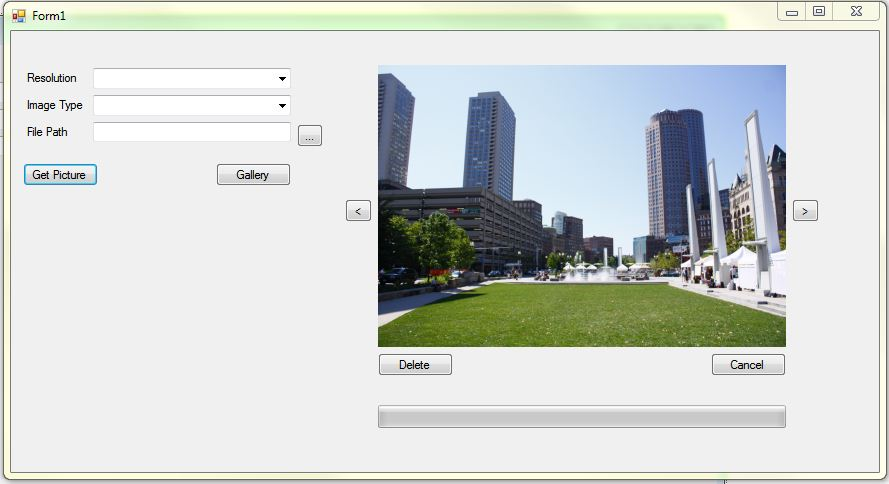
\includegraphics[scale=0.7]{initialGUI.png} 
\caption{The initial design of GUI\label{ini_GUI}}
\end{figure}

\subsubsection{Initial Class Diagram}



Figure~\ref{ini_Class} shows initial design of classes to implement. The \texttt{JPEGFileReader} Class is use for decoding the JPEG file. The decoding method is in the plan of the final program because the image take a long time to download. So, if a  The method is that in the JPEG file, there are headers. In order to make the image progressively better, these header must be extracted. The method commandCheck use check each byte of the image for a \texttt{0XFF} value. For any JPEG file, 0XFF is the start of the header of the JPEG image. The huffman table and quantization table can transform from the byte value. 
\begin{center}
\begin{figure}[!hbtp]
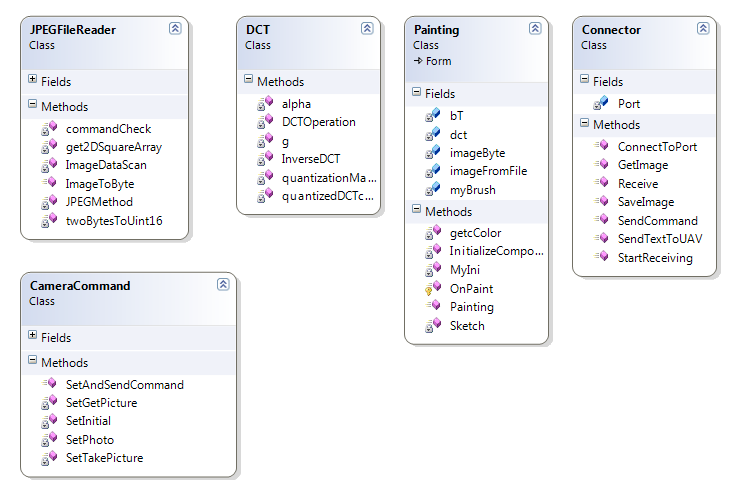
\includegraphics[width=150mm,height=100mm]{initialClassDiagram.png} 
\caption{The initial design of GUI classes\label{ini_Class}}
\end{figure}
\end{center}
DCT has many math operation and equation which have to be implemented on the image viewer program. This include discrete cosine transform, and inverse discrete cosine transform. The inverse DCT for encoding:

\begin{equation}
f_{xy}=\sum_{u=0}^7\sum_{v=0}^7 \alpha(u) \alpha(v) F_{u,v} \cos\Big[\dfrac{\pi}{8}(x+\dfrac{1}{2})u\Big]\cos\Big[\dfrac{\pi}{8}(y+\dfrac{1}{2})v\Big]
\end{equation}

$x$ is the pixel row, for the integer $0< x< 8$

$y$ is the pixel column, for the integer $0< x< 8$

$\alpha(u)$ is a normalizing scale factor

$F_{u,v}$ is the reconstructed approximate coefficient at coordinates $(u,v)$
 
$f_{x,y}$ is the reconstructed pixel at coordinates $(x,y)$

This complicated function should implement in the ground station because if the picture is encoded in the compressed way, the ground station must be able to extract it. In the end, we have to determine whether is it faster to display image normally, or to do encoding/decoding JPEG file. The another downside of this method is that there are many encoding resource which work perfectly, but because of this is long and complex, it might cause some error and time consuming.
The painting class is supported by the DCT class. The intention of this class is to display an encoded image point by point on the picture box.By this method, the pictureBox can display an image at the first pixel.
The \texttt{CameraCommand} class design for send the data from the ground station to the camera. The idea is that make the camera sync with the payload by using the ground command. \texttt{SetAndSendCommand} use for set the byte command and then send it to the payload via the Console port. \texttt{SetGetPicture,SetInitial, SetPhoto, and SetTakePicture} methods are use for setting the correct byte in order to send the byte by using \texttt{SetAndSendCommand} class.




\subsubsection{Use Case Diagram}

Figure~\ref{GUI_useCase} shows a possible user action on the program. The user can save, open and delete any jpeg image from the computer. The program can also detect the corrupted image and ask the user to delete it. The user has an option to connect to the UAV. This is incase of the UAV is not connected properly. The most important function is get picture from the UAV camera. This will send and receive complex command which will be described. The internal program will process the byte and display the information as image onto the pictureBox. The user will then have an option to save the image and close the program.
\begin{center}
\begin{figure}[!hbtp]
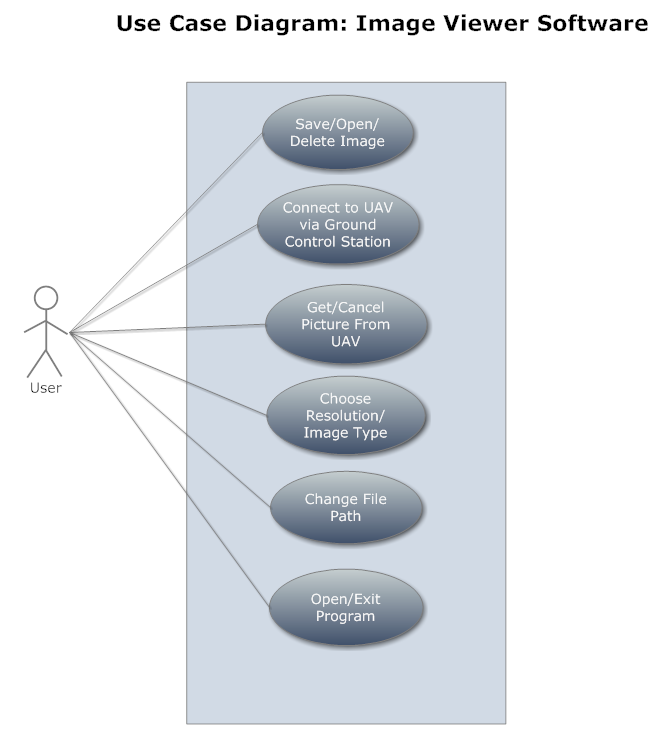
\includegraphics[scale=0.6]{userCase.PNG} 
\caption{Use case diagram of the GUI\label{GUI_useCase}}
\end{figure}
\end{center}



\subsection{Approach: Different C\# .NET Classes}
The C\# language on Microsoft Visual Basic Studio is a development environment for creating our Ground Station Image Viewer application. Choosing the right class to connect to the port helps the developer save time to program the application. The class should be able to connect to the UAV port and it must be able to send both byte and string command and receive bytes camera data from the UAV.  The C\# program has two .NET classes that can connect to port. They are SerialPort Class and Socket Class. 
\subsubsection{SerialPort Class}
The System.IO.Ports namespace contains classes for controlling serial ports. The SerialPort class is the most important one.It has ability to synchronous and event-driven I/O, access to pin and break states, and access to serial driver properties\cite{peak_netFrame}. It can change the port properties such as the stop bit, parity bit, baud rate, etc. It has handshake function that communicate to the port and report if the data or token was received successfully.
By using this class, the COM port setting has to be memorized which will be simple to load and saves from/to disk.In the process both public and private fields of the object and the name are converted to a stream of bytes.

\begin{tabular}{|p{14.5cm}|}
\hline
\texttt{SerialPort( portName, baudRate, parity bit, dataBits, StopBits ) }
\\
\hline
\end{tabular} 


The advantage of using this class is that the port can change baud rate, handshaking, parity bit, and stop bit. The class has a read and writes methods which connection with TCP/IP is possible.

Write() SerilPort's public method is use to send data of bytes to an output buffer at the specified offset

\begin{tabular}{|p{14.5cm}|}
\hline
\texttt{Read(Byte(), Int32, Int32)}
	 	Reads a number of bytes from the SerialPort input buffer and writes those bytes into a byte array at the specified offset.
	
	
\texttt{Write(Char(), Int32, Int32)} 	
Writes a specified number of characters to the serial port using data from a buffer.
	
	
\\
\hline
\end{tabular} 


 However, the implementation of the class has too many unnecessary set up and the code will be very long and can cause error. If the UAV baud rate is different from the program baud rate, the error will occur. The parity bit, and end bit and baud rate have to be setup in order to connect to the port, but these set up in UAV already.
\subsubsection{Socket Class}
The Socket is more programmer friendly, robust and a high level connection class. The socket class is use to send and receive data, in similar method as an open file allows an application to read and write data to stable storage.  It also makes a simple handshaking between the client and server machines. It can connect to multi clients, which this is necessary for a multi-port which we are using. The program can easily connect to the port by using the method:


\begin{tabular}{|p{14.5cm}|}
\hline
\texttt{Connect (String host name,Int32 port number)}
\\
\hline
\end{tabular} 

By this method, the program takes the baud rate and parity bit configuration from the UAV so the setup is the same. This class sends and array of bytes to the console port and to the data stream port by:

\begin{tabular}{|p{14.5cm}|}
\hline
\texttt{Send(byte[] command, Int32 length, SocketFlags)}
\\
\hline
\end{tabular} 


And receive data from the port by:


\begin{tabular}{|p{14.5cm}|}
\hline
\texttt{Receive(byte[] data, Int32 length, SocketFlags)}
\\
\hline
\end{tabular} 

\section{Progressive JPEG Manipulation}
Mitch

\section{Physical Implementation}
Andy


%% ----------------------------------------------------------------
\chapter{Chosen Design Approaches}
%% ----------------------------------------------------------------


\section{Payload Image Capture}

\section{Payload/Ground Station Interaction}

\section{Ground Station Image Viewer}
\subsection{.NET C\# class: Socket for the UAV Port Connector}
The socket class was the class chosen for the UAV port connector. It support TCP connection between the client and the server to do low level communication work\cite{xiaX}. The System.IO.Ports namespace has a SerialPort class that can control settings of the port such as baud rate, stop bit, parity bit, and data length. However, this become a disadvantage because the baud rate of the UAV has to be fixed according to the specification. Although it is good to set up a port, but for the software that uses an existing port, the Socket class is more useful and easier to implement by the programmer. The changes of class improve efficiency of connection between port and the program. The baud rate and extra bits are automatically adjusted to be the same as the port, so the setting is identical between the input and output. 
\subsection{GUI design}
These small software can combine to make a bigger software that can be used in the final GUI.
Implementation of the main GUI have omitted some of the buttons in the initial design. The gallery button is not needed because the left and right button is use for scrolling the whole directory of the image. The top tool strip menu has been added because this layout is familiar to any user. The image type have been removed because the raw image data makes the stream data slow and the image viewer program is not supported the file type. The priority is speed of transmitting the data from the UAV. Therefore, raw image is not the option for the user. The progress bar has moved to the button left of the page instead of displaying it below the pictureBox. This allow the application to have bigger picture box, more compact size and more professional looks. The stop button allows the user to interrupt the downloading image.

The final GUI has been planned to have many functions such as auto triggering, image type, resolution type, file path chosen, progress bar, help button, stop and delete. The GUI will be using mini application that has been implemented in the earlier stage. However, the GUI will gradually improve function by function. After all the small function has finished implemented, the final GUI can be made easily.  

The first step is to make a ''Get Picture'' function work. The plan is when the user click on the Get Picture button, the button sends a string command to the ground station software with correct command bytes. Then the customer's software will generate a command byte to the payload. Then the payload sends a ''Picture Taken'' command back through the data stream port. The GUI will then automatically send a download request command to the payload. The payload will then send image data back to the data stream port. The small programs that have been implemented in the early stage of development are reused here to send and receive data from the port. 

For a .NET C\# Programming, there is a previous tools that we can use to change directory, open and save files. The OpenFileDialog,  SaveFileDialog, and FolderBrowser dialogue are existing classes that is suitable to do this job. However, to open any file dialogue, the application needs to have a STAThread in order to handle multiple objects. STAThread is an attribute which applied to the main method, indicating that the application should communicate with unmanaged COM code using the Single Threading Apartment. It allows main thread or the main form to run in the background while the file dialogue is executing. 

These file dialogues are not stated in the image viewer specification. But it has been implemented because the user may install the program in many computers and the initial folder might not exist and this might cause the system to give an error. It is also make the users feel that they can use the program more freely.  It also give the advantage of limiting the access to only an existing file, so there is no error when trying to save the image.

\subsubsection*{GUI connection}
 When the program start running, the program initialized the port and commands the customer’s application to tell the UAV to stream data to the data stream port. Figure~\ref{GCS_connect_command} shows the connection between the UAV data stream port and the ground station. The UAV has two ports, console port, and data stream port and it can send and receive any length of data. SEND\_ ZERO\_ TOKEN is designed by the customer’s so when the DataStream port receives this handshaking token, it will start streaming data. When any data transmission and receive, the software transfer the data through pipes. There are some global initializations that the software needs to perform only once when it is loaded for the first time. Note that the console port is manually connect by the ground control station software. The image viewer will give an error when there is no connection.
 The method to stream data is by writing this code to the user program:
 
\begin{center}
\texttt{da 20 ht}
\end{center}

''da'' defines which graph on the customer's program to display the data. ''20'' define the time period to send an amount of data in millisecond. ''ht'' is the customer's defined code to show height on da graph. 


\begin{center}
\begin{figure}[!hbtp]
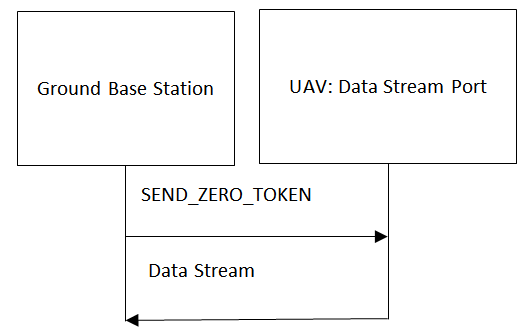
\includegraphics[scale=0.5]{connect_command.png} 
\caption{The connection of data stream port\label{GCS_connect_command}}
\end{figure}
\end{center}

\subsubsection*{GUI data flow diagram}

\begin{center}
\begin{figure}[!hbtp]
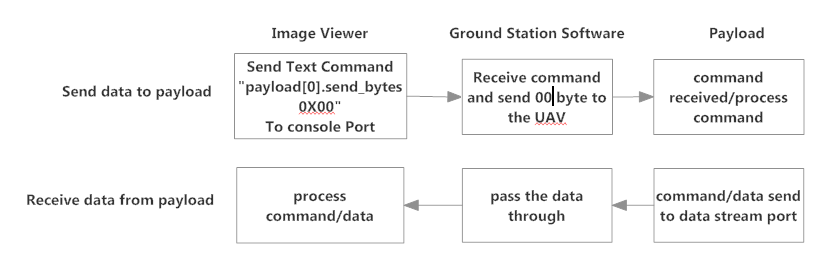
\includegraphics[scale=0.6]{GCS_Payload_communication.PNG} 
\caption{The connection of data stream port\label{GCS_Payload_comm}}
\end{figure}
\end{center}

Table~\ref{command_table} shows how the command receive and send at ground station.SEND\_ZERO\_TOKEN is use for toggle the data stream port in order to make it send data to the image viewer. TAKE\_ PICTURE command sends 0 byte to command port by sending a string command to the UAV as shown in Figure~\ref{GCS_Payload_comm}. The PICTURE\_ TAKEN signal act in a similar way to ACK (acknowledgement) command which send back to the ground with a value of number of packet of the byte data. To ensure that the number of packet is the same in ground station and the UAV, the SEND\_ DOWNLOAD\_ REQUEST command sends back the information of number of packet. The number of packet shows how many cycle does the image view to do to receive all the data.  The payload will then send the DOWNLOAD\_ INFO to the ground station which follows by the IMAGE\_ DATA. The image data consist of 3 information bytes the first byte is always 4, this number tell the image view program that it is an image data. The next 2 bytes is saying which number of packet it is. If there is any packet skipped, the image viewer program will noticed and either send error or ask the UAV for the old set of packet. The image data at each cycle have a variable length. The program is designed to take the variable length of data.

\begin{table}[!htbp]

\begin{center}
\begin{tabular}{l l @{.} l}
 Command&
\multicolumn{2}{l}{Address Byte } \\

\hline
\underline{Command from Ground} & \\
SEND\_ZERO\_TOKEN & 0 \\
TAKE\_PICTURE & 0 \\
SEND\_DOWNLOAD\_REQUEST & 2 [MSB] [LSB]  \\
\\
\underline{Command received at Ground}\\
PICTURE\_TAKEN & 1 [MSB] [LSB]\\
DOWNLOAD\_INFO & 3 [MSB] [LSB]\\
IMAGE\_DATA & 4 $\overbrace{ [packet number]}^{2bytes} \overbrace{[image data]}^{data length}$ \\
\end{tabular}
\caption{Command table\label{command_table}}
\end{center}
\end{table}

\subsection{Code Description}

\section{Physical Implementation}
Andy

%% ----------------------------------------------------------------
\chapter{Implementation}
%% ----------------------------------------------------------------


\section{Payload Image Capture}

\section{Payload Controller}

\section{Ground Station Image Viewer}
The implementation of the program needs to start from many very basic programs such as connect to the port, change byte data to image, and change image to byte. So the first prototype was implemented by using console application in order to save time while debugging and we can see the output from the UAV. In order to see that the DataStream port stream data, the UAV set to send some data on the customer’s program, and then the data will be taken through the port and so we can see from the software. Figure \ref{finalGUI} is the screen shot of the final GUI. 

\begin{center}
\begin{figure}[!hbtp]
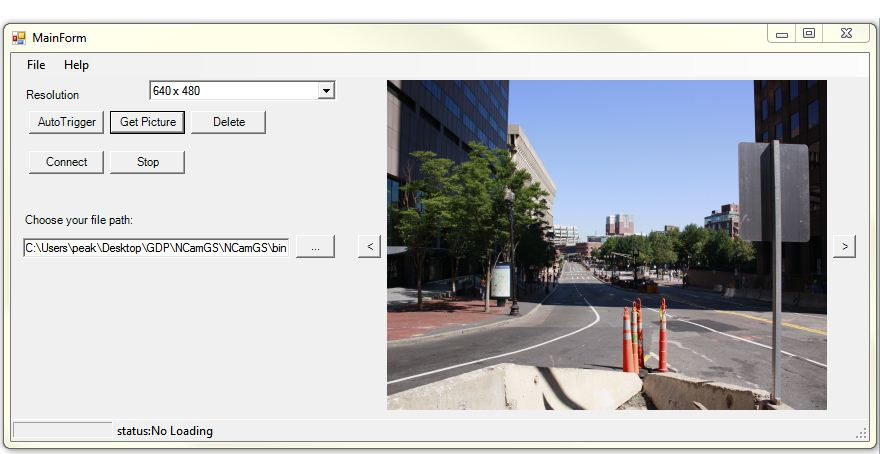
\includegraphics[scale=0.5]{finalGUI.png} 
\caption{final GUI\label{finalGUI}}
\end{figure}
\end{center}
 
\subsection{Code Highlight}

This section describe the code that is important for the program. The entire code will not be described but it will be in the appendix. In the image viewer program. It needs a class that can do these to port: connect, receive and send. FileStream class is a class in the .NET C\# which can create a file. BinaryWriter class used for writing the byte data into the generated file made by the FileStream class. The file directory will introduce a thread. While the open or save a file, the main application must be running, so the application need to deal with multi threads at the same time. Also when the get picture button got clicked, the main application is frozen because of the thread time organize do one thing at a time. The special code of thread need for handle this thread. 

\subsubsection*{Connect to UAV}
The Socket class has functions to send and receive byte and strings data. The handshaking protocol is using this code:

\begin{lstlisting}[caption={connect to port},label=lst:connectT]
public void ConnectToPort(Int32 portNumber, string portName)
{
        try            
        {
             Port.Connect(portName, portNumber);                
        }            
        catch 
        {            
            MessageBox.Show("Error code
                
             \n Unable to connect to dataStreamPort:
             \n Please check that:                
             \n1.The dataStreamPort is connected                 
             \n2.The program gcs has opened                 
             \n3.The program has connect to the dataStreamPort                
             \n4.The program has send stream data                
             \n5. The program as to run testbyte on da");                
        }            
}
        \end{lstlisting}

        
	The design of the .NET Socket class simply connect to a Port by a single command without any hesitation of changing the baud rate, stop bits, and parity bits. This advantage makes the Socket class a more useful class to work with the Port with existing and static set up. 

\subsubsection*{Start of the program}



\begin{lstlisting}[caption={Start of the program}, label=lst:payload_shared_mem_set]
	statusLabel.Text = ''Starting'';   
	progressBar.Value = 1;   
	string fileName = string.Format(''uavPictureAt { 0:yyyy-MM-dd_hh-mm-ss-tt}.jpg'', DateTime.Now);
	FileStream fileStream;
	fileStream = new FileStream(filePathTextBox.Text+''\\"+fileName, FileMode.Create);      
	BinaryWriter opFile = new BinaryWriter(fileStream);
	uavConn.SendTextToUAV("da 20 payload[0].mem_bytes[0]");      
 \end{lstlisting}
             In order to make the file name different and meaningful, the name of the picture will be the time and date of the time taken the picture. This has been done using the date and time class. fileStream was initiate to be in FileMode.Create, so it can create file. The BinaryWriter write the binary byte into a file in the directory of the fileStream. 
            
\texttt{string fileName = string.Format("uavPictureAt{ 0 : yyyy-MM-dd\_ hh-mm-ss-tt}
 .jpg", DateTime.Now);   }  
        
            This code time setting is valid for a file name. It will display year, month,date, and time in this order. The BinaryWriter class can create a binary file using specific data layout for its bytes. 

\subsubsection*{Change File Directory}
If the user wish to change the directory of the image taken, the image viewer program must support it. the mnuOpen\_click() method introduce an OpenFileDialog class. It begin with open file dialog box. This allow the user to open an inital image to the program. If the user took a picture, it will be saved in the same directory as the open file. This file dialog is limited to only the jpg picture in order to avoid the error of displaying the image. 
This file dialog introduce an extra thread. Without thread handler, the program will automatically organize the thread in the same timeline. This means it have to finish one event before it start another. The more detail about thread will be discussed in the thread section. 
\begin{lstlisting}[caption={change file directory},label=lst:changeFD]

        private void mnuOpen_Click(object sender, EventArgs e)        
        {        
             OpenFileDialog fileOpen = new OpenFileDialog();      
            
             fileOpen.Title = ''Select file to open:'';   
             fileOpen.Filter =''(* .JPG)| *.JPG; |(*.* )| *.* '';           

             if (fileOpen.ShowDialog() == DialogResult.OK)    
             {
    
                 updateDirectory(fileOpen.FileName);     
                 if (jpegList.Length != 0)     
                 {                    
                     pictureBox.Image = Image.FromFile(jpegList[filePathCount]);       
                 }         
                else       
                {       
                     pictureBox.Image = Image.FromFile(jpegList[0]);        
                }        
             }        
             pictureBox.SizeMode = PictureBoxSizeMode.StretchImage;       
             fileOpen.Dispose();        
        }       
        \end{lstlisting}
\subsubsection*{Threading}

A Scheduler that is reponsible for time-slicing threads controls the thread execution, manaing blocking of I/O message and signal handling\cite{keithC}. In any program there is always a main or initial thread running in a recursive loop that repond to the client application. In image viewer program, the main thread is the window application. When the get picture button got clicked, it will generate another less fundamental thread which will be execute after the loop have done. Therefore, in order to deal with this application while the picture is loading we need

\begin{center}
\texttt{Application.DoEvents();.}
\end{center}

During a process of taking picture and loading from the sky, the program wait for the loop to be finished before the user can do any action on the program. This is because while the code is processing, all other events wait in the queue, and it makes the program stop working. This can be fixed by using Application.DoEvents(). This code processes all of the Windows event messages that have queued up \cite{davidW}. When this code has been applied, the application can deal with other event at the same time as the code is running.


\begin{lstlisting}[caption={thread handling in the main},label=lst:threadH]
        [STAThread]        
        static void Main(string[] args)        
        {        
            mainForm.Show();
            while (true)            
            {            
                Application.DoEvents();                
            }
        	...
        \end{lstlisting}
        Application.DoEvents() in the Main function delegate that wraps the method that indicate where to start execution. The thread begin to run when the Application.DoEvents(); get called\cite{xieX}.When the file dialog try to run, the main application must be close. The [STAthread] has to be introduced in order to run multi thread at the same time. But, this doesn't mean the processor will be faster, but thread can make use of the resources that would go unused. A background thread can continue to run, while a foreground thread waits for the user input. This is called an apartment thread. 
        
\subsubsection*{Text Command}
TCP/IP protocols transfer data without modifying them. This allow the application to freely encode the data.\cite{davidB}.The Ground station software allow the program to send a stream of string in bytes and it will read the command bytes and send it to the payload on the UAV. The code has shown the way to implement the string and send a byte array to the payload.
	
	

\begin{lstlisting}[caption={send text in byte array},label=lst:sendT]
	 public void SendTextToUAV(string textToUAV)	        
         {        
             char[] toUAVChar = new char[512];       
             byte[] toUAVByte = new byte[512];        
             byte[] fromUAVByte = new byte[1000];       
             byte[] oneByteArray = new byte[1];       
             textToUAV += '' $\backslash$ n'';        
             toUAVChar = textToUAV.ToCharArray();        
             toUAVByte = System.Text.Encoding.ASCII.GetBytes(toUAVChar);       
             try       
             {      
                 int sendByte = consolePort.Send(toUAVByte, toUAVChar.Length, SocketFlags.None);     
             }     
            catch (SocketException ex)      
            {       
                Console.WriteLine(''ERROR\: '' + ex.Message);       
            }       
         }
\end{lstlisting}
                

To send text, the string of characters is translated into an array of bytes. American Standard Code for Information Interchange(ASCII) is use for translating English into a binary code. In the System.Text classes provide converting mechanism between each character sets. The ASCIIEncoding.GetBytes() is used for convert character array into a byte array.  
The Socket.Send() Method allow the user to send byte stream to the port connected.The customer's program will read from the port and display it onto the command line. The ''@ '' sign indicate that the command correctly sent from the application to the ground station software. The advantage of linking to the ground station software is that our customers can understand what is going on in the console line. For example:

\begin{center}
uavConn.SendTextToUAV(''da 20 payload[0].mem\_ bytes[0]'')\;
\end{center}

The text ''da 20 payload[0].mem\_ bytes[0]'' will be converted to char array and then to byte array. The byte array will then send the command to the console port to the payload by \texttt{consolePort.Send(toUAVByte, toUAVChar.Length)}. The customer is familiar with the ground station software program, so this method of sending data is satisfy. 

\subsubsection*{I/O Streams}
    The .NET framework's stream class is use as a powerful tools for encoding and decoding\cite{davidB}. In the image viewer program, we use FileStream to create a directory and to save the byte data into image. However, the program might have to deal with a corrupted image data. Framing is the problem of the receiver failed to find the beginning and the end of the message. The solution is the data packet give the information of how many loop must the program do in order to receive all the image data. The packet address locate in the second and third byte of the image data stream. 
     

\begin{lstlisting}[caption={writing binary file},label=lst:writingb]          
	for (int i = 3; i < packetSize; i++)
	{
          opFile.Write(packet[i]);
          numBytes++;
    	}
\end{lstlisting}         

       At every cycle of the data being received, opFile.Write() method will write the packet data into the file in the directory. After the cycle finished, the file will be saved and the image will be displayed in the picture box. 
    
    
\subsubsection*{Other functions}
The user might want to delete some unwanted photo, so the delete button have been implemented. The delete button work like a normal file deleting button. But it has been complicated because the photo to delete must be the photo on the pictureBox. There is an error because the photo is using by the pictureBox. To fix this problem, the picture have to shifted left or right first and then delete the photo. This will solve almost all the problem. But where there is only one picture in the file, the program can not delete because even the pictureBox is set to null, it's last memory is still point at the deleting file. However, the disadvantage of the delete button is that if the wanted photo got deleted accidentally, it might take a long time to launch the UAV again and take the same photo.
%insert combobox of resolution in zoom in level

The camera has options of resolution. This can be useful when the speed is important. The lower the resolution, the faster the data transmitted to the ground. GUI has the combo box for the user to choose any wanted resolution in the options. The resolution allow user to have more accessible to the camera. However, this mean there is more on the programmer side to program the application.
%zoom in or progress bar image

The baud rate that we can transmit data from the UAV is 38.4kbaud. Bandwidth limitations severely restrict the volume of data to transfer over the wireless link. It takes around 8 to 20 seconds to transmit an image of resolution 640x480. This progress bar tells the user how much percentage of data received. The progress bar update at each cycle of the data receives. At the end of each image downloaded, the progress bar reset to its normal state.  The status text tells the user what signal have been sent or received. This status text ensures that the picture is downloading and it is good for testing that the tasking in process. These two nice application allocate on the bottom left of the GUI. However, these have to implement every cycle of the data collection and it might cause the cycle to run slower. The actual loop is much faster than the 38.4kbaud, therefore there is no problem implementing these in.

\subsection{Final Use Case Diagram}
%describe what changes compare to the first use case diagram
\begin{center}
\begin{figure}[!hbtp]
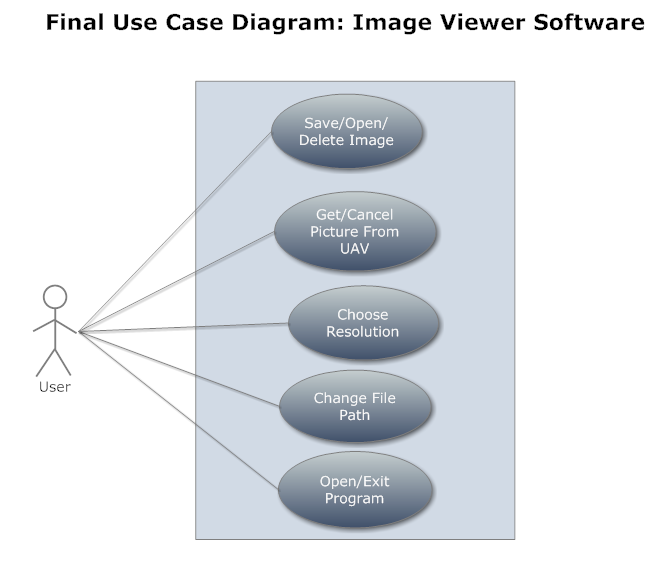
\includegraphics[scale=0.7]{FinaluserCase.PNG} 
\caption{Final use case diagram of the GUI\label{GUI_finalUseCase}}
\end{figure}
\end{center}


\subsection{Work Flow Diagram}
Describe Work Flow
%describe what changes compare to the first use case diagram
\begin{center}
\begin{figure}[!hbtp]
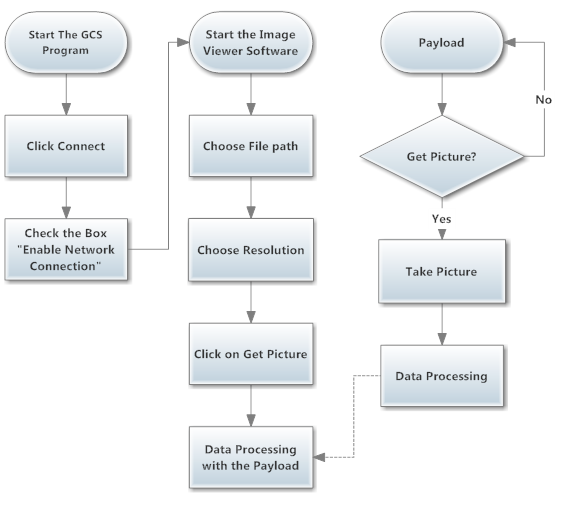
\includegraphics[scale=1]{finalWorkFlow.PNG} 
\caption{Final use case diagram of the GUI\label{GUI_finalWorkFlow}}
\end{figure}
\end{center}
\section{Progressive JPEG Manipulation}

\section{Physical Implementation}

\section{System Integration}


%% ----------------------------------------------------------------
\chapter{Overview}
%% ----------------------------------------------------------------
An overview of the entire project process goes here...

\section{Final Deliverables}
The final deliverables of the project are described here...

\section{Evaluation Against Specification}


%% ----------------------------------------------------------------
\chapter{Testing}
%% ----------------------------------------------------------------

\subsection{Camera/Payload Interaction}

\subsection{SD Card/Payload Interaction}

\subsection{Payload/Ground Station Interaction}

\subsection{Ground Station Image Viewer}

\subsection{Progressive JPEG Manipulation}

%% ----------------------------------------------------------------
\chapter{Project Management}
%% ----------------------------------------------------------------
Project management goes here...

\section{Gantt Charts}
Michael
Place Gantt charts here.

\section{Risk Management}
Mitch
Place risk management considerations and compare with risks encountered.

\section{Work Allocation}
Peak
Talk about planned work allocation to be compared with actual work allocation. Reflect on efficiency.

\subsection{Planned Work Allocation}
Talk about the tasks planned and the skills audit.

\subsection{Actual Task Allocation}
Talk about who did what in the end and how tasks were passed around. How did people work together?

\section{Team Resources}
John
What we used to get the job done...

\subsection{Budget}
What did we need to buy in the end?

\subsection{Electronic Material}
Did we make use of anything electronic that we had before the project?

\section{Group Communication}
Andy
Talk about how the group contacted each other (email, meetings, mobiles)...

\subsection{Formal Meetings}
Talk about the usefulness and benefit of the formal Tuesday meetings...

\subsection{Methods of Communication}
Talk about which methods were used more often, which were useful...

\subsection{Software Management}
How we used e-mails, SVN Tortoise, and Github to keep our progress safe...


%% ----------------------------------------------------------------
\chapter{Future work}
%% ----------------------------------------------------------------
Future work goes here. May be combined with the Evaluation section.

%% ----------------------------------------------------------------
\chapter{Evaluation}
%% ----------------------------------------------------------------

\section{Success}
Discuss how successful the final project is in terms of meeting the project brief goals...

\section{Team}
Discuss how successful the team functioned as a whole? Well communicated? Tasks properly assigned? Sufficient work done?

%% ----------------------------------------------------------------
\chapter{Conclusions}
%% ----------------------------------------------------------------
Conclusions go here.

%% ----------------------------------------------------------------
\chapter{Documentation}
%% ----------------------------------------------------------------
Mitch
All supplementary documentation prepared for the project can be referenced here...

%% ----------------------------------------------------------------
\acknowledgements{I would like to thank...}
\dedicatory{To \dots}

%% ----------------------------------------------------------------
\include{Introduction}
\include{Conclusions}
\appendix
\backmatter
\chapter{Glossary}

\section*{Terms} 
\begin{description}
	\item[YCbCr] Colour space used to represent JPEG images. Composed of three values:
		\begin{description}
			\item[Y] luma component.
			\item[Cb] blue-difference chroma component.
			\item[Cr] red-difference chroma component.
		\end{description}
	\item[4:x:y]Chroma subsampling notation.
		\begin{description}
			\item[4] Luma horizontal (and vertical) sampling reference.
			\item[x] Cb and Cr horizontal sampling factor.
			\item[y] Cb and Cr horizontal sampling factor. If 0, indicates 2:1 vertical subsampling for both Cb and Cr.
		\end{description}
\end{description}

\section*{Abbreviations} 
\begin{description}
	\item[AC] Alternating Current 
	\item[DC] Digital Current 
	\item[JPEG] Joint Photographic Experts Group, creators of the jpeg compression method. Used interchangeably with the jpeg image type.
	\item[EXIF] EXchangeable Image File format for digital still cameras.
	\item[MCU] Minimum Coded Unit
	\item[DFT] Discrete Fourier Transform
	\item[FFT] Fast Fourier Transform
	\item[DCT] Discrete Cosine Transform
	\item[WHT] Walsh–Hadamard Transform
	\item[KLT] Karhunen-Lo\`eve Transform
	\item[SOI] Start Of Image
	\item[SOF] Start Of Frame
	\item[DHT] Define Huffman Table(s)
	\item[HT] Huffman Table
	\item[DQT] Define Quantization Table(s)
	\item[QT] Quantization Table
	\item[SOS] Start Of Scan
	\item[EOI] End Of Image
	\item[SD card]
\end{description}
\chapter{Appendix A}

\bibliographystyle{ecs}

\begin{thebibliography}{9}

	\bibitem{tortorella_jpeg_enc} Tortorella, Richard. \emph{Image Doctoring: JPEG Encoding and Analysis}. Rep. NARCAP, May 2009. Web. 11 Oct. 2011. \url{http://www.narcap.org/reports/narcap_IR-01_DigHoaxing.pdf}.
	
	\bibitem{exif_std} Japan Electronics and Information Technology Industries Association (JEITA). \emph{Digital Still Camera Image File Format Standard (Exchangeable Image File Format for Digital Still Cameras: Exif)} Version 2.1. Tech. Japan Electronic Industry Development Association (JEIDA), 12 June 1998. Web. 14 Oct. 2011 \url{http://www.exif.org/Exif2-1.PDF}.
	
	\bibitem{netravali_digital_repr} Netravali, Arun N., and Barry G. Haskell. \emph{Digital Pictures: Representation and Compression}. New York: Plenum, 1988. Print. 
	
	\bibitem{jpeg_layout} \emph{JPEG File Layout and Format}. Original URL: \\http://www.funducode.com/freec/Fileformats/format3/format3b.htm (defunct).\\DCube Software Technologies, 5 July 2002. Web. 28 Oct. 2011. \url{http://class.ee.iastate.edu/ee528/Reading%20material/JPEG_File_Format.pdf}
	
	\bibitem{winzip_jpeg_compression} WinZip® International LLC. \emph{JPEG Compression}. Tech. Version 1.0. 11 Sept. 2008. Web. 28 Oct. 2011. \url{http://www.winzip.com/wz_jpg_comp.pdf}.
	
	\bibitem{poynton_chroma_subsampling} Poynton, Charles. \emph{Chroma Subsampling Notation.} Charles Poynton. 24 Jan. 2008. Web. 31 Oct. 2011. \url{http://poynton.com/PDFs/Chroma_subsampling_notation.pdf}.
	
	\bibitem{kerr_chroma_subsampling} Kerr, Douglas A. \emph{Chrominance Subsampling in Digital Images}. Rep. Issue 2. 3 Dec. 2009. Web. 31 Oct. 2011. \url{http://dougkerr.net/pumpkin/articles/Subsampling.pdf}.
	
	\bibitem{hass_impulse_jpeg} Hass, Calvin. \emph{ImpulseAdventure - Digital Photography Articles.} 2008. Web. 22 Nov. 2011. \url{http://www.impulseadventure.com/photo/}.
	
	\bibitem{peak_netFrame} C.D. CĂLEANU, V. TIPONUŢ, I. BOGDANOV, S. IONEL, I. LIE \emph{C\# and .NET Framework for uC communication protocol Proceedings of the 11th WSEAS International Conference on COMPUTERS, Agios Nikolaos, Crete Island, Greece, July 26-28, 2007
implementation} 2008. Web. 22 Nov. 2011.
\url{www.wseas.us/e-library/conferences/2007cscc/papers/561-338.pdf}.

	\bibitem{tsuiK} Kakit Tsui \emph{Ad Hoc Network:Generic USB Device Driver Development} (2003)
\url{http://crisp.ece.cornell.edu/mengproj/alan_report.doc}.

	\bibitem{keithC} Keith Clark,Peter J. Robinson,Richard Hagen.(2001) Multi-threading and message communication in Qu-Prolog.\textit{Theory and Practice of Logic Programming} . 1 (3), p283-301 
	
		\bibitem{davidW} Keith Clark,Peter J. Robinson,Richard Hagen.(2004) \textit{Beginning .NET game programming in C\#.} United States of America: Apress. 

		\bibitem{xieX} Xiaoyun Xie.(2004) \textit{Distributed Objects System in C\#.} Rochester, United States of America. 

		\bibitem{davidB} David B. Makofske, Michael J. Donahoo, Kenneth L. Calvert.(2004) \textit{TCP/IP sockets in C\#  practical guide for programmers}. Amsterdam: Elsevier.

\end{thebibliography}
\end{document}
%% ----------------------------------------------------------------
